\chapter{Effektive Bandbreite}

Zur quantitativen Analyse des frequenzabhängigen Übertragungsverhaltens des Messsystems wurde das Verstärkungsprofil der HLE-Box über einen breiten Frequenzbereich hinweg untersucht. 
Die Verstärkung $G(f)$ bestimmt, wie Eingangssignale unterschiedlicher Frequenz vom System übertragen oder unterdrückt werden, und muss daher exakt bekannt sein. 
Die Filterstufen in der HLE-Box begrenzen das Spektrum der durchgelassenen Signale und beeinflussen somit die effektive Rauschleistung am Ausgang. 
Die relevante Größe zur Beschreibung dieser spektralen Selektion ist die frequenzabhängige Verstärkung \cite{praktikum}: 

\begin{equation}
  G(f) = \frac{\mathrm{RMS}_{\mathrm{out}}}{\mathrm{RMS}_{\mathrm{in}}},
\end{equation}

welche als Funktion der Frequenz gemessen wurde.

Die HLE-Box enthält konfigurierbare Butterworth-Filter zweiter Ordnung in Form eines Tiefpassfilters und eines Hochpassfilters. 
In dieser Messung wurden die Grenzfrequenzen auf $f_l = \SI{10}{\kilo\hertz}$ (Tiefpass) bzw.\ $f_h = \SI{1}{\kilo\hertz}$ (Hochpass) eingestellt, sodass sich ein Bandpassverhalten ergibt. 
Die frequenzabhängige Verstärkung der einzelnen Filterstufen ergibt sich aus \cite{praktikum}:

\begin{align}
  G_{\mathrm{LP}}(f) &= \biggl[1 + \Bigl(\frac{f}{f_l}\Bigr)^4\biggr]^{-\frac{1}{2}}, \\
  G_{\mathrm{HP}}(f) &= \Bigl(\frac{f}{f_h}\Bigr)^2 \,\biggl[1 + \Bigl(\frac{f}{f_h}\Bigr)^4\biggr]^{-\frac{1}{2}},
\end{align}

Die Verstärkung berechnet sich als Produkt \cite{praktikum}:

\begin{equation}
  G(f) = G_{\mathrm{LP}}(f)\,G_{\mathrm{HP}}(f).
\end{equation}

Daraus ergibt sich die effektive Bandbreite als Integral über das Quadrat der Gesamtverstärkung \cite{praktikum}:

\begin{equation}
\begin{aligned}
\Delta f_{\mathrm{eff}}
  &= \int_{0}^{\infty} G^2(f)\,\mathrm{d}f
   = \int_{0}^{\infty} G_{\mathrm{LP}}^2(f)\,G_{\mathrm{HP}}^2(f)\,\mathrm{d}f \\[6pt]
  &= \int_{0}^{\infty}
    \bigl[1 + \bigl(\tfrac{f}{f_L}\bigr)^4\bigr]^{-1}
    \bigl(\tfrac{f}{f_H}\bigr)^4
    \bigl[1 + \bigl(\tfrac{f}{f_H}\bigr)^4\bigr]^{-1}
    \,\mathrm{d}f \\[6pt]
  &= \frac{\sqrt{2\pi}\,f_L^4}{4\,(f_H + f_L)\,(f_H^2 + f_L^2)}.
\end{aligned}
\end{equation}

Die schematische Darstellung des Messaufbaus ist in \cref{fig:schaltfrequenz} dargestellt. 
Ein sinusförmiges Eingangssignal wurde von einem Funktionsgenerator erzeugt und an die HLE-Box angelegt. 
Die RMS-Eingangs- und Ausgangsspannungen wurden mit einem Zweikanal-Oszilloskop über einen logarithmisch verteilten Frequenzbereich hinweg aufgenommen. 
Die gemessenen Werte sind in \cref{tab:freq_response} aufgeführt, und der resultierende Verstärkungsverlauf $G(f)$ ist in \cref{fig:gvsf} dargestellt.


\begin{figure}[htbp]
    \centering
    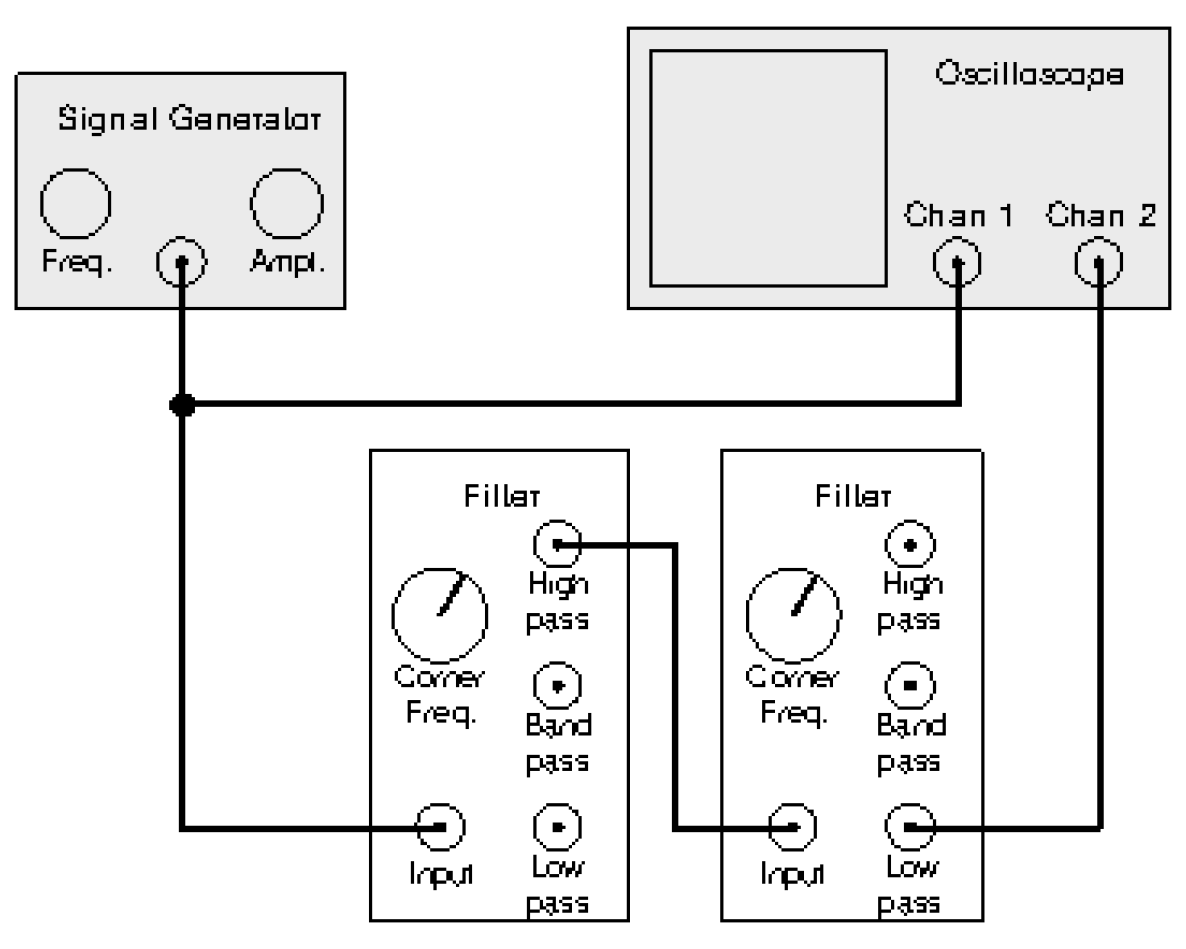
\includegraphics[width=0.5\textwidth]{figs/schalt frequenz.png}
    \caption{Schaltplan zur Messung des Ansprechverhaltens der Frequenzfilter \cite{praktikum}}
    \label{fig:schaltfrequenz}
\end{figure}

\begin{table}[H]
\centering
\resizebox{0.35\columnwidth}{!}{%
  \begin{tabular}{|c|c|c|}
    \hline
    $f\,/\,\si{\Hz}$ & $\mathrm{RMS}_{\mathrm{in}}\,/\,\si{\V}$ & $\mathrm{RMS}_{\mathrm{out}}\,/\,\si{\V}$ \\ \hline
    $2 \pm 0.006$          & $19.8 \pm 0.1$   & $0.660 \pm 0.010$ \\ \hline
    $8 \pm 0.024$          & $54.9 \pm 0.1$   & $0.780 \pm 0.010$ \\ \hline
    $20 \pm 0.06$          & $70.0 \pm 0.1$   & $0.720 \pm 0.010$ \\ \hline
    $80 \pm 0.24$          & $74.5 \pm 0.1$   & $1.05 \pm 0.01$   \\ \hline
    $200 \pm 0.6$          & $74.9 \pm 0.1$   & $3.05 \pm 0.01$   \\ \hline
    $800 \pm 2.4$          & $75.1 \pm 0.1$   & $40.3 \pm 0.01$  \\ \hline
    $2000 \pm 6$           & $75.2 \pm 0.1$   & $73.0 \pm 0.01$  \\ \hline
    $8000 \pm 24$          & $75.2 \pm 0.1$   & $63.7 \pm 0.01$  \\ \hline
    $20000 \pm 60$         & $75.0 \pm 0.1$   & $18.5 \pm 0.01$  \\ \hline
    $80000 \pm 240$        & $74.1 \pm 0.1$   & $1.50 \pm 0.01$  \\ \hline
    $200000 \pm 600$       & $74.0 \pm 0.1$   & $0.915 \pm 0.010$\\ \hline
    $800000 \pm 2400$      & $74.1 \pm 0.1$   & $0.910 \pm 0.010$\\ \hline
    $2000000 \pm 6000$     & $74.2 \pm 0.1$   & $0.900 \pm 0.010$\\ \hline
    $8000000 \pm 24000$    & $81.0 \pm 0.1$   & $0.810 \pm 0.010$\\ \hline
    $10000000 \pm 30000$   & $68.7 \pm 0.1$   & $0.890 \pm 0.010$\\ \hline
  \end{tabular}%
}
\caption{Gemessene RMS-Eingangs- und Ausgangsspannungen (mit Unsicherheiten) als Funktion der Frequenz.}
\label{tab:freq_response}
\end{table}

\begin{figure}[htbp]
    \centering
    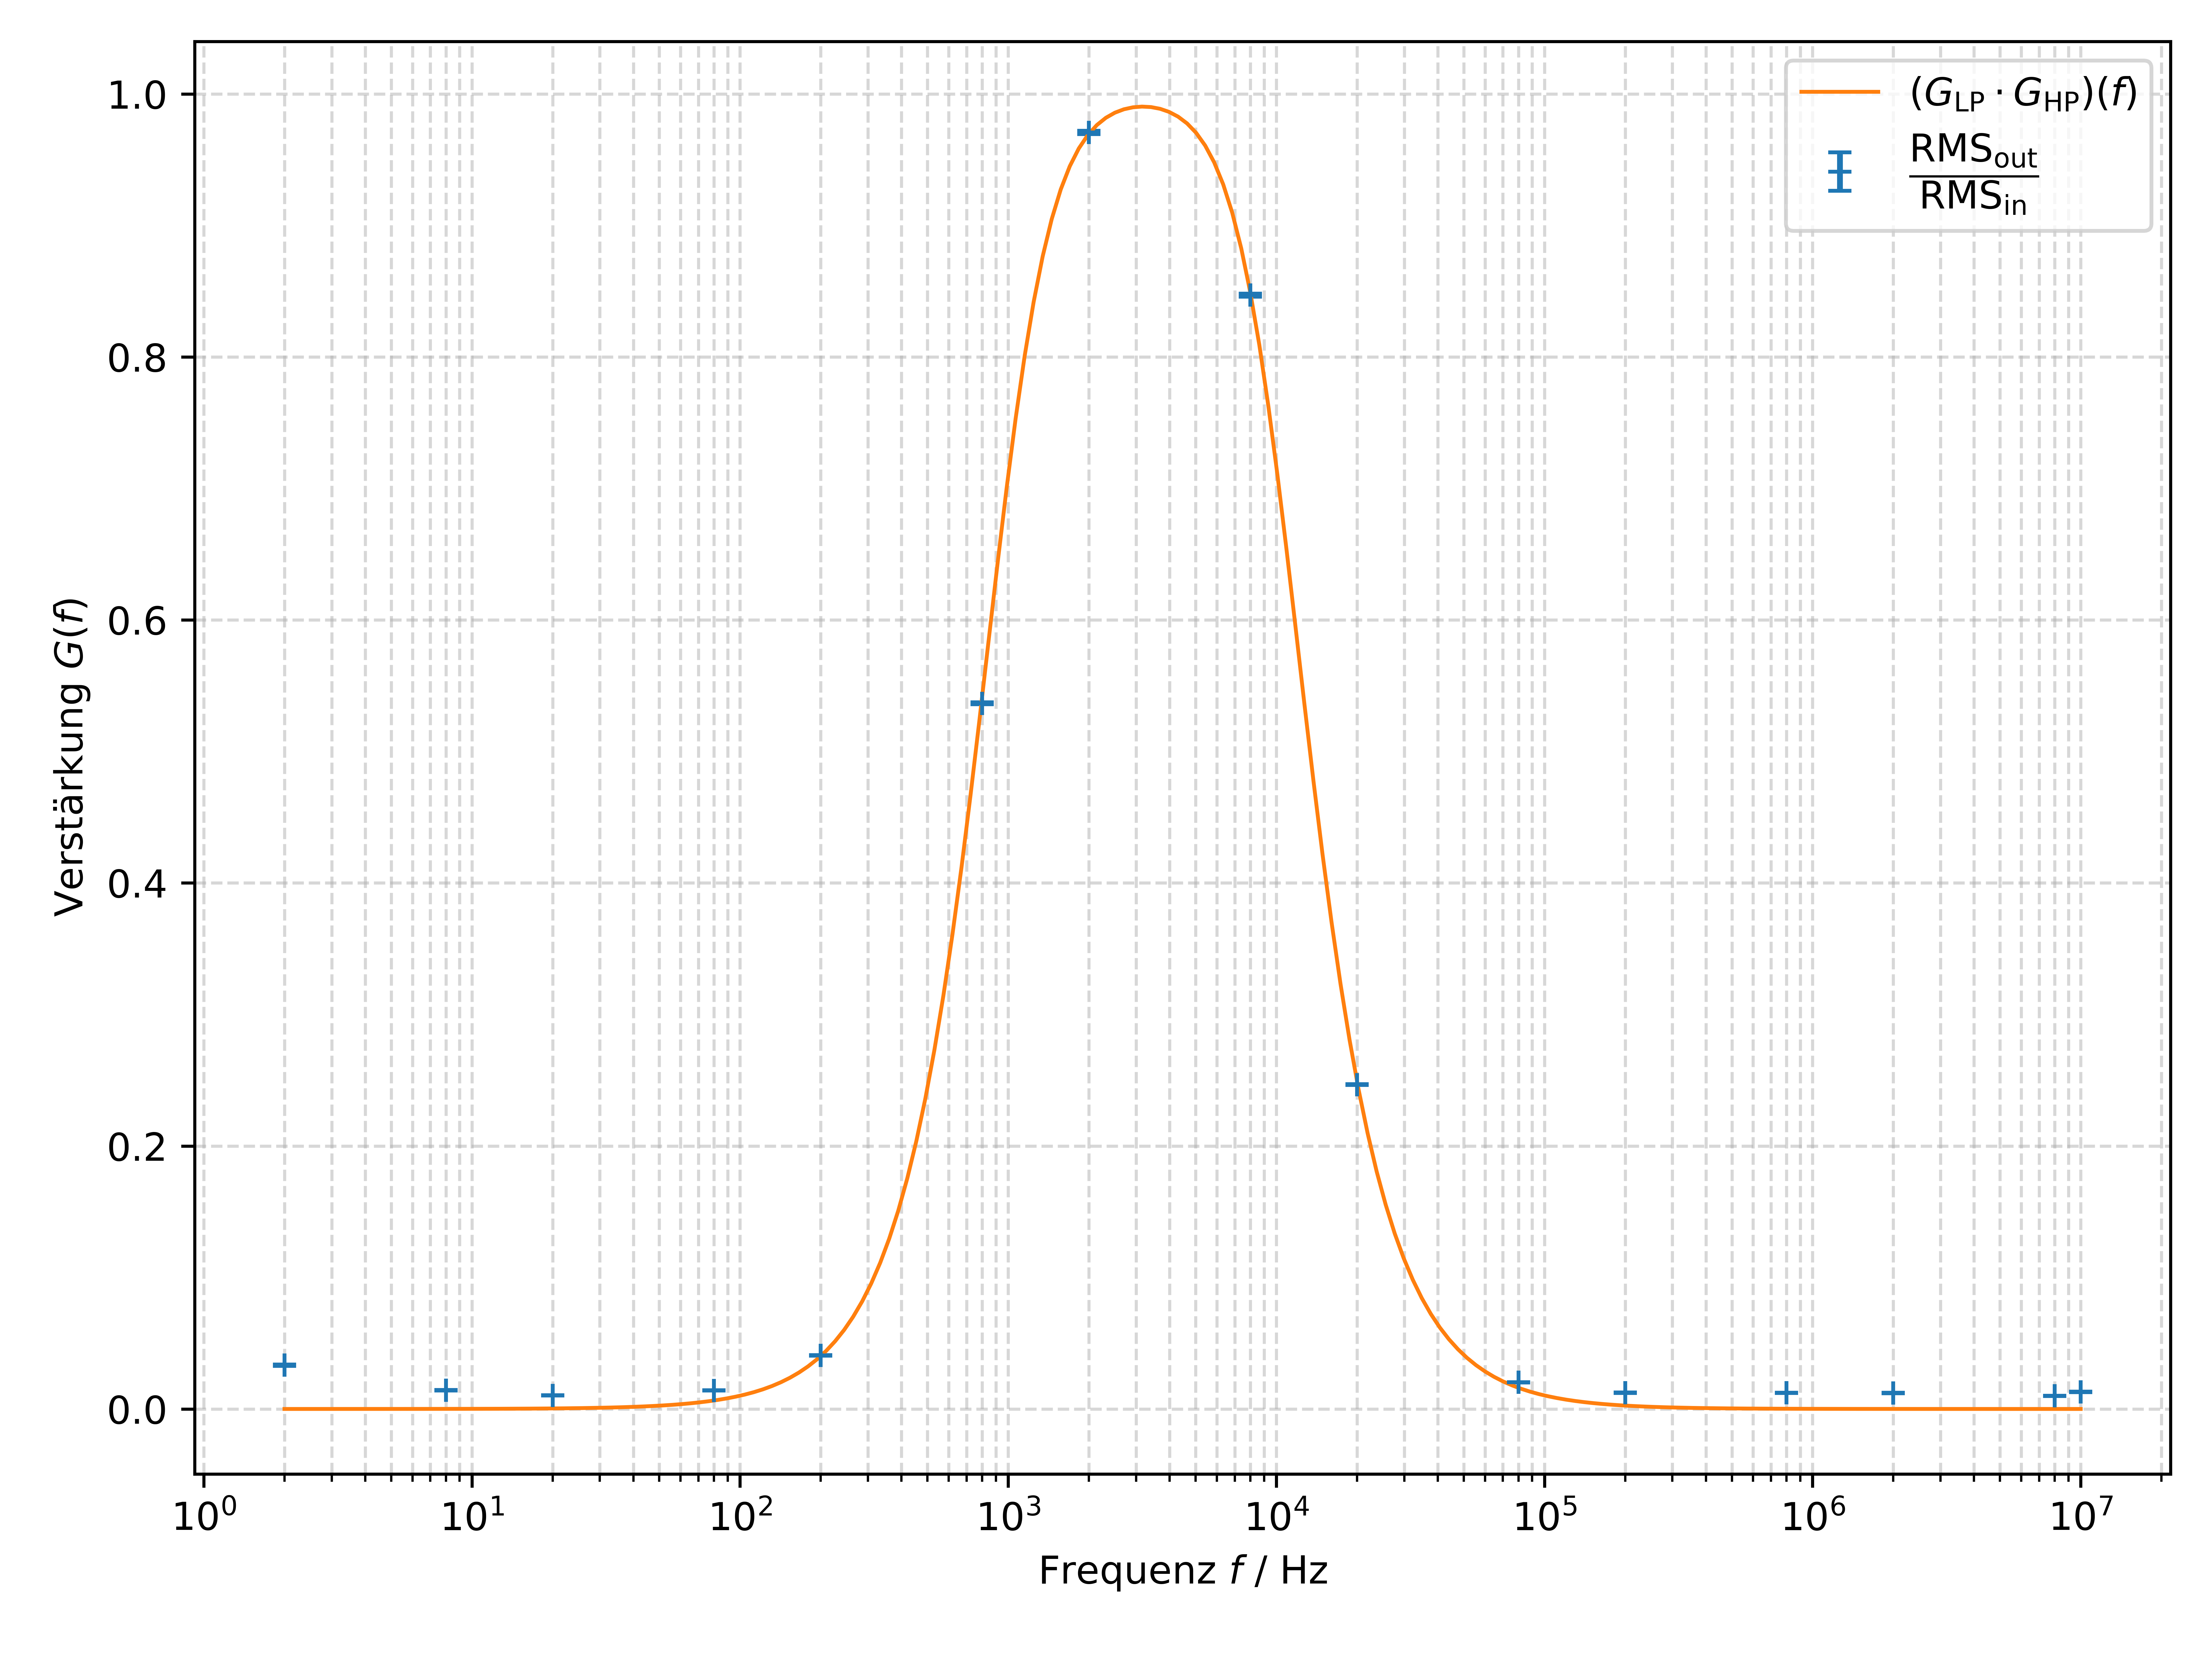
\includegraphics[width=0.75\textwidth]{figs/Gvsf.png}
    \caption{Diagramm der Verstärkung $G(f)$ gegen die Frequenz $f$. Experimentelle Datenpunkte ($\mathrm{RMS}_{\mathrm{out}}/\mathrm{RMS}_{\mathrm{in}}$) sind mit Fehlerbalken dargestellt, und die durchgezogene Linie repräsentiert das theoretische Modell $(G_{\mathrm{LP}}\cdot G_{\mathrm{HP}})(f)$. Werte sind in \cref{tab:experimental_gains}}

    \label{fig:gvsf}
\end{figure}

Die gemessene frequenzabhängige Verstärkung $G(f)$, bestimmt aus dem Verhältnis der RMS-Ausgangs- zur RMS-Eingangsspannung, zeigt eine ausgezeichnete Übereinstimmung mit der theoretisch erwarteten Kurve, welche durch das Produkt der individuellen Butterworth-Filterantworten $G_{\mathrm{LP}}(f)\cdot G_{\mathrm{HP}}(f)$ beschrieben wird. 
Diese Übereinstimmung wird in \cref{fig:gvsf} deutlich, wo die experimentellen Daten über mehrere Dekaden hinweg eng an die theoretische Funktion anschließen. 
Aufgrund der hohen Präzision bei der Spannungsmessung sind die statistischen Unsicherheiten der Datenpunkte vernachlässigbar klein und im Diagramm nicht sichtbar.

An den Frequenzgrenzen - unterhalb von etwa $100\,\mathrm{Hz}$ und oberhalb von $100\,\mathrm{kHz}$ - treten systematische Abweichungen vom theoretischen Verstärkungsverlauf auf. 
Diese können auf parasitäre Einflüsse wie mechanische Vibrationen oder Netzbrumm ($50\, \mathrm{Hz}$) im niederfrequenten Bereich sowie aufelektromagnetische Störungen im Hochfrequenzbereich (z.\,B. Einkopplung von Rundfunkwellen) zurückgeführt werden. 
Da diese Effekte im theoretischen Modell nicht berücksichtigt sind, führen sie vermutlich zu kleinen, systematischen Abweichungen in der gemessenen Verstärkung außerhalb der nominellen Durchlassbandbreite.

Im Bereich zwischen den gewählten Grenzfrequenzen $f_h = 1\,\mathrm{kHz}$ und $f_l = 100\,\mathrm{kHz}$ folgt das Filterverhalten jedoch sehr präzise der theoretischen Vorhersage. 
In diesem Intervall ist die Extrapolation der Verstärkungsfunktion $G(f)$ auf Grundlage der vorliegenden Messdaten als physikalisch gerechtfertigt anzusehen. 
Die daraus berechnete effektive Bandbreite $\Delta f_{\mathrm{eff}}$ kann somit als verlässlich angenommen werden.

Eine nichtlineare Kleinste-Quadrate-Anpassung ($\chi^2$) der theoretischen Übertragungsfunktion $G(f)=G_{\mathrm{LP}}(f)\cdot G_{\mathrm{HP}}(f)$ an die gemessenen Daten ergab die Filterparameter

\begin{equation}
  f_l = (10144{,}66 \pm 7{,}24)\,\mathrm{Hz}, 
  \quad
  f_h = (996{,}30 \pm 0{,}83)\,\mathrm{Hz}.
\end{equation}

Diese Werte stimmen hervorragend mit den nominalen Hardware-Einstellungen der HLE-Box überein, die für eine Tiefpass-Grenzfrequenz nahe $f_l = 10\,\mathrm{kHz}$ und eine Hochpass-Grenzfrequenz nahe $f_h = 1\,\mathrm{kHz}$ konfiguriert war. 
Die daraus bestimmte effektive Bandbreite des Bandpasses ergab sich zu

\begin{equation}
  \Delta f_{\mathrm{eff}} = 5733{,}42\,\mathrm{Hz}.
\end{equation}

Obwohl der reduzierte Chi-Quadrat-Wert der Anpassung

\begin{equation}
  \chi^2/\mathrm{dof} = 4163{,}56
  \quad
  \bigl(\chi^2 = 54126{,}27,\ \mathrm{dof} = 13\bigr)
\end{equation}

deutlich größer als eins ist, ist dies in erster Linie auf die extrem kleinen statistischen Unsicherheiten der RMS-Spannungsmessungen zurückzuführen, die zu einer hohen Empfindlichkeit des Anpassungskriteriums führen. 
Dennoch beschreibt die gefittete Kurve das gemessene Verstärkungsverhalten über den gesamten Frequenzbereich sehr genau, insbesondere im Durchlassbereich. 
Daher gelten die extrahierten Grenzfrequenzen und die effektive Bandbreite als physikalisch sinnvoll und quantitativ zuverlässig für weitere Analysen.
